\newpage
\section{Consuntivi di periodo}

In base ai consuntivi di periodo dei periodi completati sono state effettuate le diverse modifiche per rientrare nel budget preventivato al momento della consegna per aggiudicarci il capitolato.

\subsection{\PD}
La differenza di ore da quelle preventivate nella sezione 4 di questo documento a quelle effettivamente fatte è la seguente:

\begin{table}[h]
	\begin{center}
		\begin{tabular}{|c|c|c|c|c|}
			\hline
			\textbf{Ruolo}	& \textbf{Ore Preventivate} & \textbf{Differenza ore} & \textbf{Costo} & \textbf{Differenza costo}\\
			\hline
			\Pm &	7  & 0 &	210 &	0\\
			\hline
			\Am	&	7 &	0 & 140 & 0\\
			\hline
			\Prog	&	76 & -11 & 1672 & -242 \\
			\hline
			\Ver &	38 & +4 & 570 & +60\\
			\hline
			\textbf{totale}	&	\textbf{128} & \textbf{-7} & \textbf{2592} & \textbf{-182} \\
			\hline
		\end{tabular}
	\end{center}
	\caption{Consuntivo di periodo \PD}
\end{table}

\begin{figure}[H]
	\centering 
	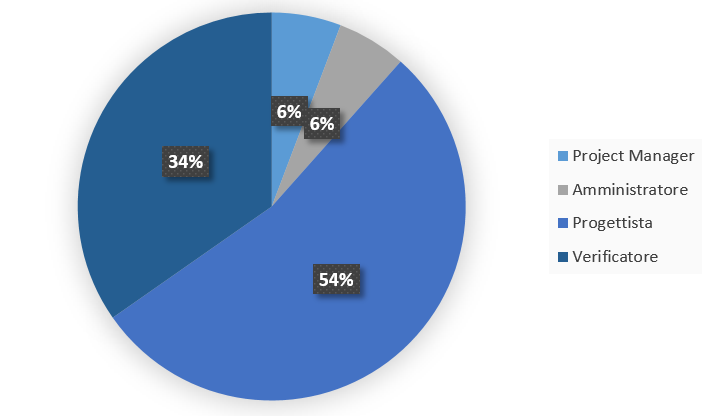
\includegraphics[scale=1.25]{Immagini/Consuntivo/ConsuntivoPD.png}
	\caption{Consuntivo delle ore per ruolo, \PD}
\end{figure}

Dal consuntivo di periodo, dunque, emerge un \textbf{risparmio di 182 euro} rispetto ai costi preventivati in precedenza.

\newpage

\subsection{\COD}
La differenza di ore da quelle preventivate nella sezione 4 di questo documento a quelle effettivamente fatte è la seguente:

\begin{table}[h]
	\begin{center}
		\begin{tabular}{|c|c|c|c|c|}
			\hline
			\textbf{Ruolo}	& \textbf{Ore Preventivate} & \textbf{Differenza ore} & \textbf{Costo} & \textbf{Differenza costo}\\
			\hline
			\Pm &	0  & 0 &	0 & 0\\
			\hline
			\Am	&	0 & 0 & 0 & 0\\
			\hline
			\Prog	&	0 & 0 & 0 & 0 \\
			\hline
			\Ver &	0 & 0 & 0 & 0\\
			\hline
			\textbf{totale}	&	\textbf{0} & \textbf{0} & \textbf{0} & \textbf{0} \\
			\hline
		\end{tabular}
	\end{center}
	\caption{Consuntivo di periodo \COD}
\end{table}

Dal consuntivo di periodo, dunque, emerge un \textbf{...} rispetto ai costi preventivati in precedenza.
